\documentclass[a4paper,10pt]{article}
\usepackage[utf8x]{inputenc}
\usepackage{verbatim}
\usepackage{graphicx}
\usepackage{enumerate}

%opening
\title{Lab 4}
\author{William Richard}

\begin{document}

\maketitle

\section{Verbose Startup}
  \begin{center}
  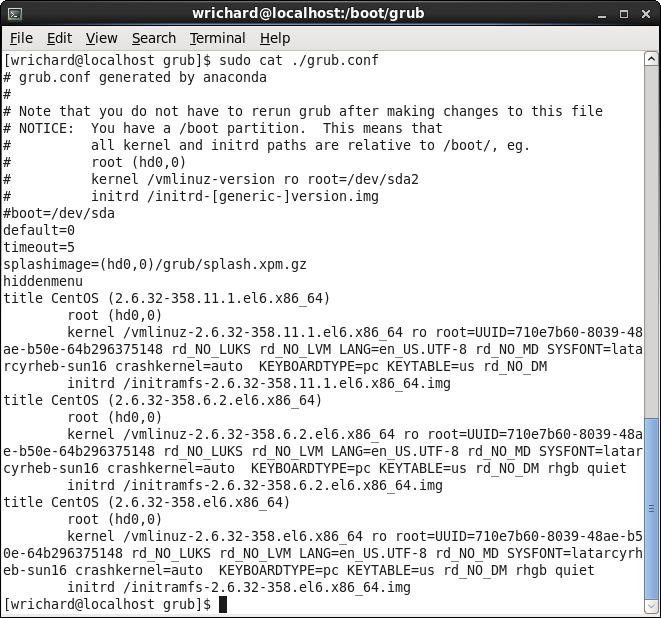
\includegraphics[width=\linewidth]{./verbose-grubconf.png}
  \end{center}

\section{Drive Dmesg}
I don't think my virtual machine had any IDE drives, so none appear in the dmesg output
  \begin{center}
  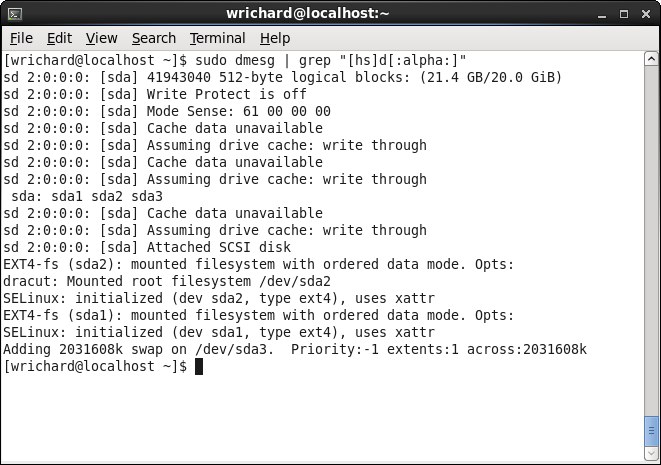
\includegraphics[width=\linewidth]{./dmesg-drives.png}
  \end{center}

\section{CLI login}
  \begin{center}
  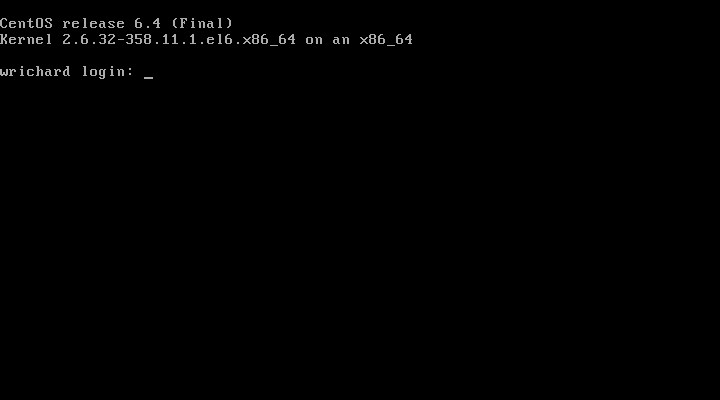
\includegraphics[width=\linewidth]{./cli.png}
  \end{center}

\section{psk.sh}
\subsection{code}
\verbatiminput{psk.sh}
\subsection{screenshot}
  \begin{center}
  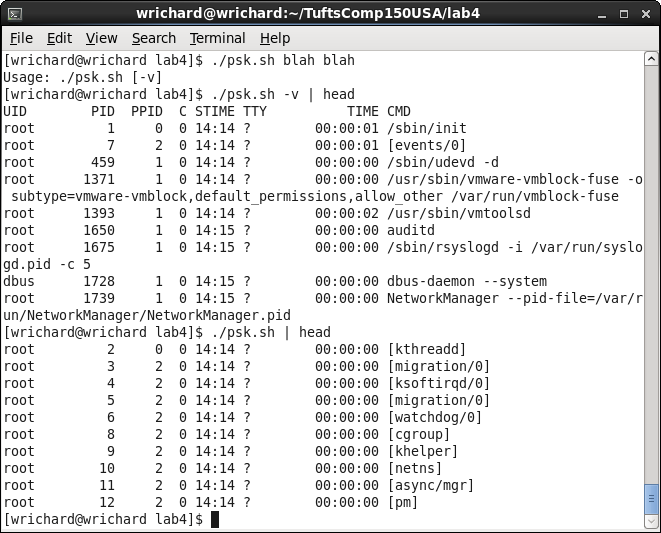
\includegraphics[width=\linewidth]{./psk.png}
  \end{center}

\section{chkconfig}
  \begin{center}
  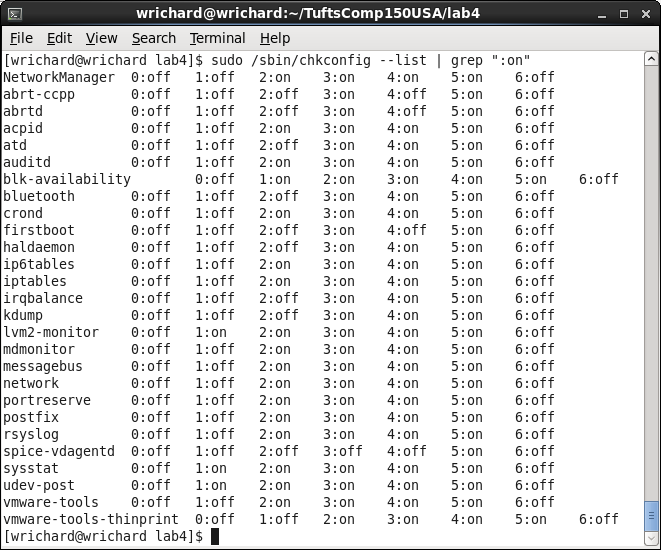
\includegraphics[width=\linewidth]{./chkconfig.png}
  \end{center}

\section{bootlog}
\subsection{code}
\verbatiminput{bootlog.sh}
\subsection{screenshot}
  \begin{center}
  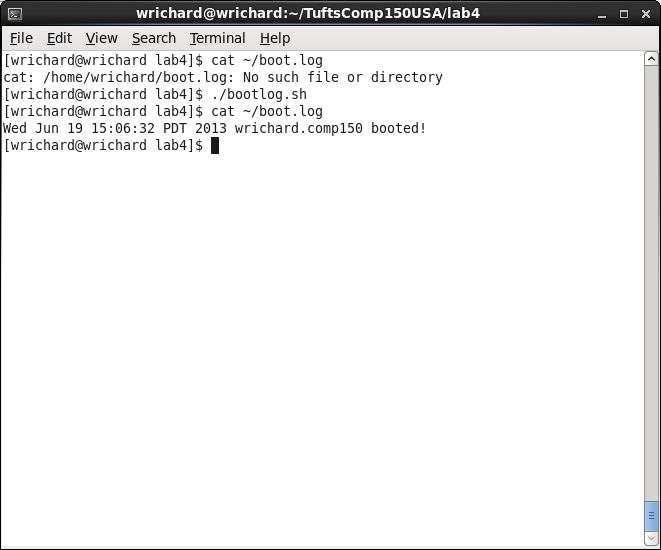
\includegraphics[width=\linewidth]{./bootlog.png}
  \end{center}

\section{rc.local}
  \begin{center}
  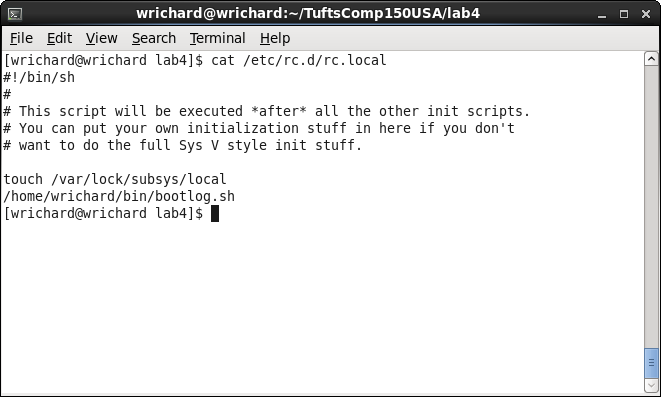
\includegraphics[width=\linewidth]{./rclocal.png}
  \end{center}











\end{document}




\section{p139 E5.2}
\begin{enumerate}[(a)]
  \item The output of top or ps, sorted by cpu usage or memory usage, quickly and easily reveal processes that are hogging resources.
  \item 
\begin{verbatim}
kill -s STOP -p <pid>
\end{verbatim}
  \item 
\begin{verbatim}
kill -s CONT -p <pid>
\end{verbatim}
  \item I would send the TERM signal - this allows the process to die gracefully.
\begin{verbatim}
kill -s TERM -p <pid>
\end{verbatim}
If I needed to guaranee that the process died, I would send the KILL signal, or signal 9, which forces tho process to die, and does not allow it to try to exit gracefully.
\begin{verbatim}
kill -s KILL -p <pid>
\end{verbatim}
\end{enumerate}

\section{ps -ef $|$ grep bash $|$ grep -v grep}
  \begin{center}
  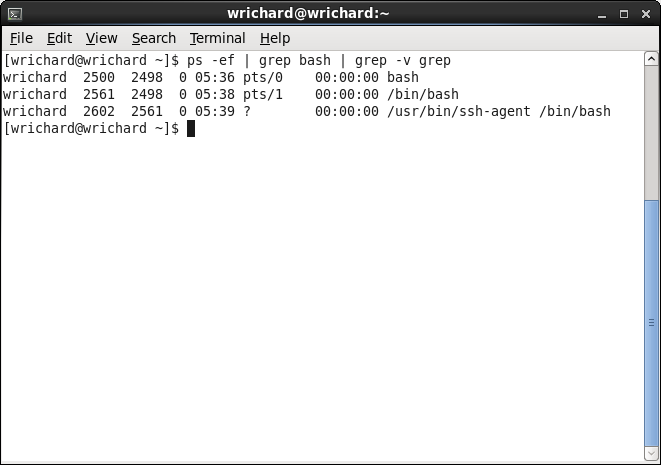
\includegraphics[width=\linewidth]{./grepbash.png}
  \end{center}

\section{find\_proc.sh}
\subsubsection{Code}
\verbatiminput{find_proc.sh}
\subsection{screenshot}
  \begin{center}
  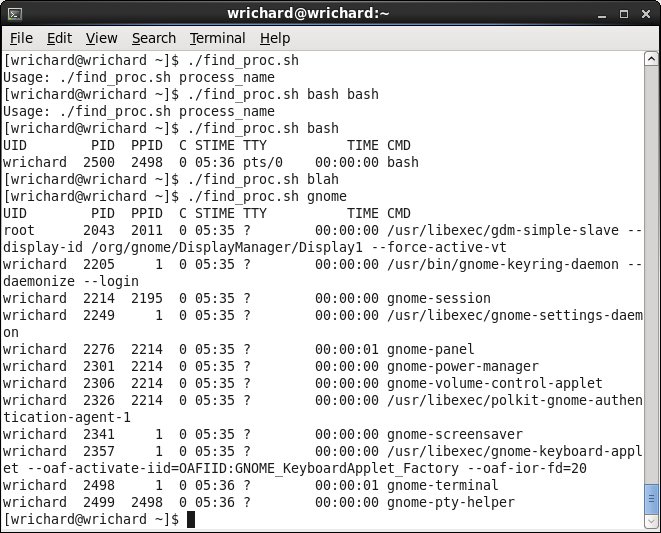
\includegraphics[width=\linewidth]{./find_proc.png}
  \end{center}

\section{top}
\subsection{sorted by memory usage}
  \begin{center}
  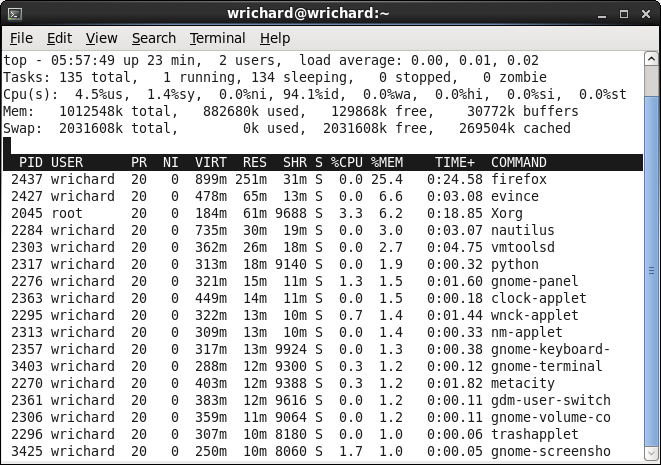
\includegraphics[width=\linewidth]{./topm.png}
  \end{center}
\subsection{two infinite processes}
  \begin{center}
  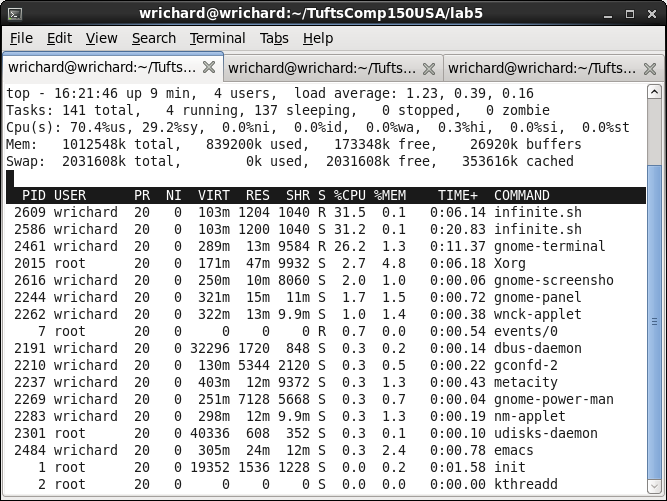
\includegraphics[width=\linewidth]{./top_infinite.png}
  \end{center}
\subsection{nice infinite process}
  \begin{center}
  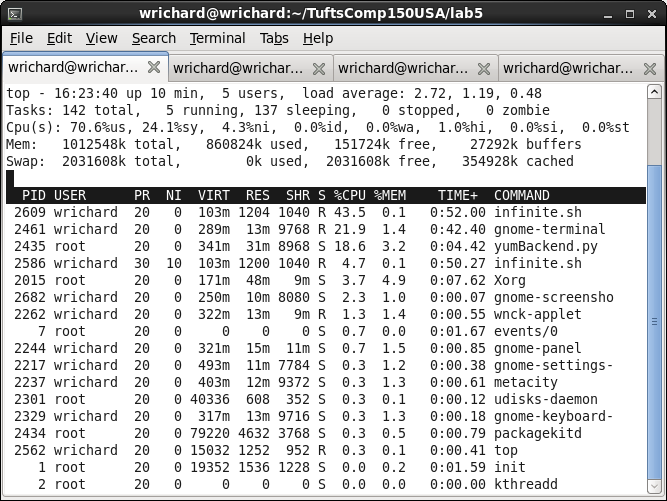
\includegraphics[width=\linewidth]{./top_nice_infinite.png}
  \end{center}

\section{login.sh}
\subsection{code}
\verbatiminput{login.sh}
\subsection{screenshot}
  \begin{center}
  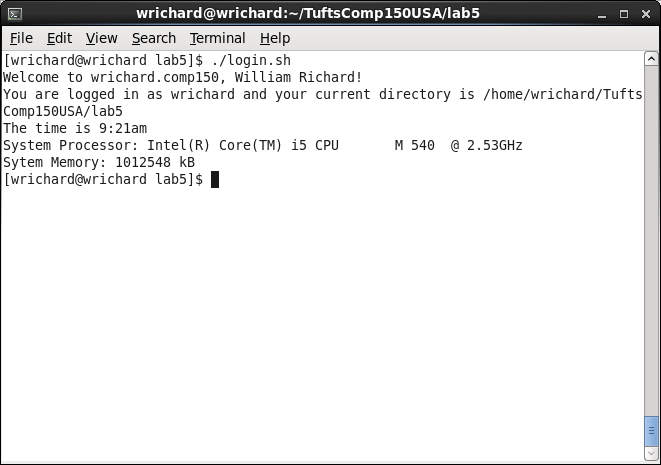
\includegraphics[width=\linewidth]{./login.png}
  \end{center}

\end{document}
